\begin{description}[leftmargin=0.7cm,style=nextline]
\item[Szenario K0:]
Der Client erstellt einen Adressbucheintrag \\
\item[Szenario K1:]
Der Client erstellt einen Adressbucheintrag .\\
\item[Szenario K2:]
Der Client erstellt einen Adressbucheintrag .\\
\item[Szenario K3:]
Der Client erstellt einen Adressbucheintrag
\end{description}
%
In den obigen Szenarien \ldots
% \begin{figure}[H]
%   \centering
%   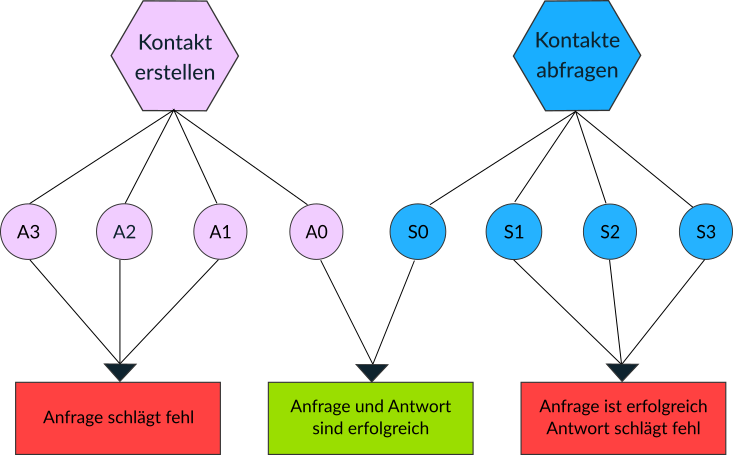
\includegraphics[width=0.8\textwidth]{Szenarien}
%   \grayRule
%   \caption[Szenarien]{Szenarien und Fälle}
%   \label{fig:scenarios}
% \end{figure}
%
% ERGEBNIS
%
\subsubsection*{Ergebnis}
